\addcontentsline{toc}{subsection}{Sideways Shooters}
\LARGE \circled{5} \textbf{Sideways Shooters} \normalsize

{\itshape A very peculiar bandit ritual}

The greatest group standoff in the wild, wild west draws near. 
The red and blue factions of the sideways shooters, both sworn enemies, are bringing their best to form an interlocking spectacle.
What makes these factions special? 
Not only do they fire two pistols at the same time, but they're always pointed to the left and to the right. Take a look at the angles:

% Picture showing bandit at 0, 45, 90, 135 degree angles
\begin{figure}[h]
    \centering
    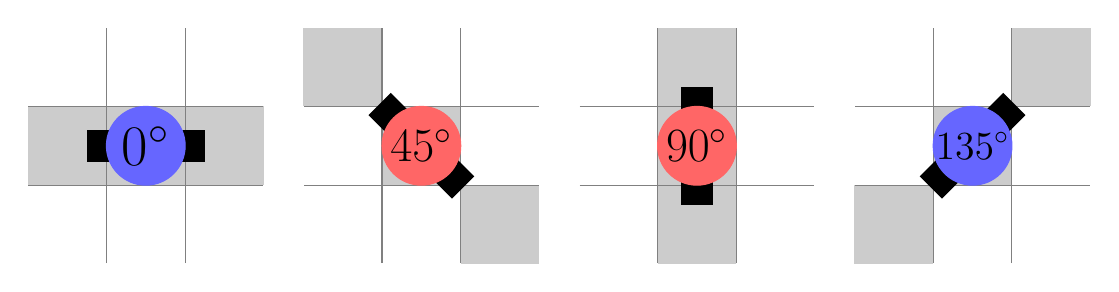
\begin{tikzpicture}
        % Draw danger areas
        \fill[gray!40!white, shift={(0, 0)}] (0, 1) rectangle (3, 2);
        \fill[gray!40!white, shift={(3.5, 0)}] (0, 2) rectangle (1, 3);
        \fill[gray!40!white, shift={(3.5, 0)}] (1, 1) rectangle (2, 2);
        \fill[gray!40!white, shift={(3.5, 0)}] (2, 0) rectangle (3, 1);
        \fill[gray!40!white, shift={(7, 0)}] (1, 0) rectangle (2, 3);
        \fill[gray!40!white, shift={(10.5, 0)}] (0, 0) rectangle (1, 1);
        \fill[gray!40!white, shift={(10.5, 0)}] (1, 1) rectangle (2, 2);
        \fill[gray!40!white, shift={(10.5, 0)}] (2, 2) rectangle (3, 3);

        % Draw grids
        \draw[step=1cm, gray, thin] (0.01, 0.01) grid (2.99, 2.99);
        \draw[step=1cm, gray, thin, xshift=3.5cm] (0.01, 0.01) grid (2.99, 2.99);
        \draw[step=1cm, gray, thin, xshift=7cm] (0.01, 0.01) grid (2.99, 2.99);
        \draw[step=1cm, gray, thin, xshift=10.5cm] (0.01, 0.01) grid (2.99, 2.99);

        % Draw bandit 'arms'
        \fill[black] (0.75, 1.3) rectangle (1.25, 1.7);
        \fill[black] (1.75, 1.3) rectangle (2.25, 1.7);
        \fill[black, shift={(3.5,0)}, rotate around={-45:(1.5, 1.5)}] (0.75, 1.3) rectangle (1.25, 1.7);
        \fill[black, shift={(3.5,0)}, rotate around={-45:(1.5, 1.5)}] (1.75, 1.3) rectangle (2.25, 1.7);
        \fill[black, shift={(7,0)}, rotate around={90:(1.5, 1.5)}] (0.75, 1.3) rectangle (1.25, 1.7);
        \fill[black, shift={(7,0)}, rotate around={90:(1.5, 1.5)}] (1.75, 1.3) rectangle (2.25, 1.7);
        \fill[black, shift={(10.5,0)}, rotate around={45:(1.5, 1.5)}] (0.75, 1.3) rectangle (1.25, 1.7);
        \fill[black, shift={(10.5,0)}, rotate around={45:(1.5, 1.5)}] (1.75, 1.3) rectangle (2.25, 1.7);

        % Draw Bandit
        \filldraw[blue!60!white] (1.5, 1.5) circle (0.5cm) node[text=black] {\huge $0^\circ$};
        \filldraw[red!60!white] (5, 1.5) circle (0.5cm) node[text=black] {\LARGE $45^\circ$};
        \filldraw[red!60!white] (8.5, 1.5) circle (0.5cm) node[text=black] {\LARGE $90^\circ$};
        \filldraw[blue!60!white] (12, 1.5) circle (0.5cm) node[text=black] {\Large $135^\circ$};

        % Add Captions
    \end{tikzpicture}
\end{figure}


You're in charge of the showdown, and you call the shots - you can choose to rotate or remove any bandit member in the planned standoff.
Ultimately, you want to include as many bandits and duels as possible... while minimising friendly fire!

\vspace{8pt}
\hrule

\textbf{Input}

The first line of the input contains two space-separated integers $r$ and $b$, denoting the number of red and blue bandits respectively.

The next $r + b$ lines of the input will consist of three space-separated integers, giving info about each of the red and blue bandits. For bandit $i$:
\begin{itemize}
    \item The first two $(x_i,y_i)$ are the grid coordinates of the bandit.
    \item The third $\theta_i$ is the angle of the bandit, as a multiple of $45^\circ$ increments.
\end{itemize}
The first $r$ of these lines describe the red bandits; the other $b$ describe the blue bandits.

\textbf{Constraints}

\begin{equation*}
    r, b \geq 0 \text{ and } 1 \leq r+b \leq 9 \cdot 10^4 \qquad \forall i \quad 1 \leq x_i,y_i \leq 3 \cdot 10^2 \text{ and } \theta_i \in \{0, 45, 90, 135\}
\end{equation*}

\textbf{Output}

The first output line should be an integer $0 \leq k \leq r + b$, the number of bandits in your modified standoff.

The next $k$ output lines should consist of three space-separated integers - representing the x-position, y-position, and new rotation of a bandit you'd like to include in the standoff.

\vspace{8pt}
\hrule

\textbf{Scoring}

Points will be awarded to your modified standoff as follows:
\begin{itemize}
    \item \textbf{+5} for each bandit kept in the standoff.
    \item \textbf{+3} for each bandit who is pointing their pistols at one opponent.
    \item \textbf{+10} for each bandit who is pointing their pistols at two opponents.
    \item \textbf{-1} for each $45^\circ$ bandit rotation that is made from the original standoff.
    \item \textbf{-15} for each instance of a bandit pointing at a member of their own faction.
\end{itemize}

\newpage

\vspace{8pt}
\hrule

\textbf{Example}

\begin{table}[h]
    \centering
    \begin{tabular}{|p{0.4\linewidth}|p{0.4\linewidth}|}
        \hline
        Input & Output \\
        \hline
        \textbf{3 2}
        \newline 4 1 0
        \newline 2 3 135
        \newline 1 4 0
        \newline 1 1 45 
        \newline 4 3 90
        &  
        \textbf{4} 
        \newline 4 1 0
        \newline 1 4 0
        \newline 1 1 45
        \newline 4 3 90
        \\
        \hline
    \end{tabular}
\end{table}

To help explain, let's label the input and output bandits on a diagram:

\begin{figure}[h]
    \centering
    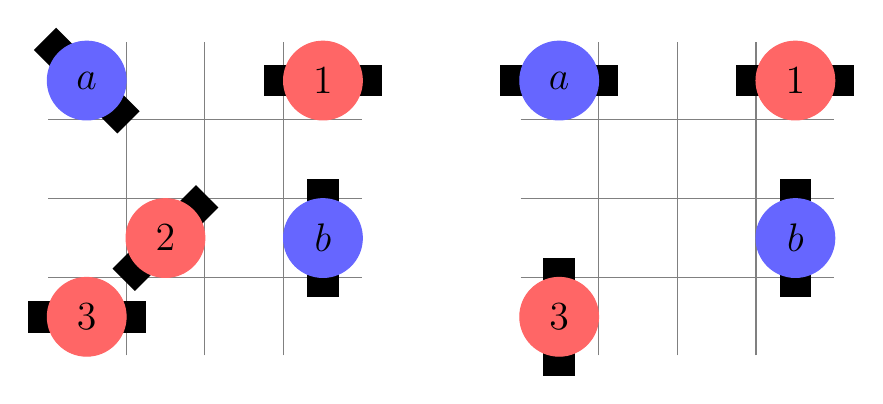
\begin{tikzpicture}
        % Draw danger areas

        % Draw grids
        \draw[step=1cm, gray, thin] (0.01, 0.01) grid (3.99, 3.99);
        \draw[step=1cm, gray, thin, xshift=6cm] (0.01, 0.01) grid (3.99, 3.99);

        % Before
        % Red 1
        \fill[black, shift={(3.5,3.5)}, rotate around={0:(0, 0)}] (-0.75, -0.2) rectangle (-0.25, 0.2);
        \fill[black, shift={(3.5,3.5)}, rotate around={0:(0, 0)}] (0.25, -0.2) rectangle (0.75, 0.2);
        \filldraw[red!60!white] (3.5, 3.5) circle (0.5cm) node[text=black] {\Large $1$};
        % Red 2
        \fill[black, shift={(1.5,1.5)}, rotate around={45:(0, 0)}] (-0.75, -0.2) rectangle (-0.25, 0.2);
        \fill[black, shift={(1.5,1.5)}, rotate around={45:(0, 0)}] (0.25, -0.2) rectangle (0.75, 0.2);
        \filldraw[red!60!white] (1.5, 1.5) circle (0.5cm) node[text=black] {\Large $2$};
        % Red 3
        \fill[black, shift={(0.5,0.5)}, rotate around={0:(0, 0)}] (-0.75, -0.2) rectangle (-0.25, 0.2);
        \fill[black, shift={(0.5,0.5)}, rotate around={0:(0, 0)}] (0.25, -0.2) rectangle (0.75, 0.2);
        \filldraw[red!60!white] (0.5, 0.5) circle (0.5cm) node[text=black] {\Large $3$};
        % Blue a
        \fill[black, shift={(0.5,3.5)}, rotate around={-45:(0, 0)}] (-0.75, -0.2) rectangle (-0.25, 0.2);
        \fill[black, shift={(0.5,3.5)}, rotate around={-45:(0, 0)}] (0.25, -0.2) rectangle (0.75, 0.2);
        \filldraw[blue!60!white] (0.5, 3.5) circle (0.5cm) node[text=black] {\Large $a$};
        % Blue b
        \fill[black, shift={(3.5,1.5)}, rotate around={90:(0, 0)}] (-0.75, -0.2) rectangle (-0.25, 0.2);
        \fill[black, shift={(3.5,1.5)}, rotate around={90:(0, 0)}] (0.25, -0.2) rectangle (0.75, 0.2);
        \filldraw[blue!60!white] (3.5, 1.5) circle (0.5cm) node[text=black] {\Large $b$};

        % After
        % Red 1
        \fill[black, shift={(9.5,3.5)}, rotate around={0:(0, 0)}] (-0.75, -0.2) rectangle (-0.25, 0.2);
        \fill[black, shift={(9.5,3.5)}, rotate around={0:(0, 0)}] (0.25, -0.2) rectangle (0.75, 0.2);
        \filldraw[red!60!white] (9.5, 3.5) circle (0.5cm) node[text=black] {\Large $1$};
        % Red 3
        \fill[black, shift={(6.5,0.5)}, rotate around={90:(0, 0)}] (-0.75, -0.2) rectangle (-0.25, 0.2);
        \fill[black, shift={(6.5,0.5)}, rotate around={90:(0, 0)}] (0.25, -0.2) rectangle (0.75, 0.2);
        \filldraw[red!60!white] (6.5, 0.5) circle (0.5cm) node[text=black] {\Large $3$};
        % Blue a
        \fill[black, shift={(6.5,3.5)}, rotate around={0:(0, 0)}] (-0.75, -0.2) rectangle (-0.25, 0.2);
        \fill[black, shift={(6.5,3.5)}, rotate around={0:(0, 0)}] (0.25, -0.2) rectangle (0.75, 0.2);
        \filldraw[blue!60!white] (6.5, 3.5) circle (0.5cm) node[text=black] {\Large $a$};
        % Blue b
        \fill[black, shift={(9.5,1.5)}, rotate around={90:(0, 0)}] (-0.75, -0.2) rectangle (-0.25, 0.2);
        \fill[black, shift={(9.5,1.5)}, rotate around={90:(0, 0)}] (0.25, -0.2) rectangle (0.75, 0.2);
        \filldraw[blue!60!white] (9.5, 1.5) circle (0.5cm) node[text=black] {\Large $b$};
        
    \end{tikzpicture}
\end{figure}

If we didn't modify the original standoff, here's how we'd score:
\begin{itemize}
    \item +5 (x5) for 5 bandits
    \item +3 (x2) for $b$ pointing at $1$, and $1$ pointing at $a$
    \item -15 (x2) for $2$ pointing at both $1$ and $3$
\end{itemize}
This would give a total of \textbf{1 Point}.

For the modified standoff on the right, here's how we'd score:
\begin{itemize}
    \item +5 (x4) for 4 bandits
    \item +3 (x4) for $b \rightarrow 1$, $1 \rightarrow a$, $a \rightarrow 1$, $3 \rightarrow a$
    \item -1 (x3) for rotating $a$ by $45^\circ$ and rotating $3$ by $90^\circ$  ($2 \times 45$)
\end{itemize}
This would give a total of \textbf{29 Points}.

Can you do better?